\documentclass[homework]{IEEEtran}
\IEEEoverridecommandlockouts
% The preceding line is only needed to identify funding in the first footnote. If that is unneeded, please comment it out.
\usepackage{cite}
\usepackage{CJKutf8}
\usepackage{indentfirst}
\usepackage{amsmath,amssymb,amsfonts}
\usepackage{algorithmic}
\usepackage{graphicx}
\usepackage{textcomp}
\usepackage{xcolor}
\usepackage{hyperref}
\usepackage[justification=centering]{caption}
\setlength{\parindent}{2em}
\def\BibTeX{{\rm B\kern-.05em{\sc i\kern-.025em b}\kern-.08em
    T\kern-.1667em\lower.7ex\hbox{E}\kern-.125emX}}
\begin{document}

\title{Homework of Pattern classification III\\
{\footnotesize \textsuperscript{*}Name: Xue Yuan  | Student number: 202228015926034}
}

\author{}
\maketitle

\begin{abstract}
This document is about the first homework for Pattern classification by \LaTeX.
\end{abstract}

\section{Short Answers and Descriptions}
\begin{CJK}{UTF8}{gkai}
$\mathbf{Q1}$: 请对反向传播算法的训练步骤进行总结;结合三层网络给出不超过三个有关权重更新的公式,
并用文字描述所述公式的含义;指出哪些因素会对网络的性能产生影响。 \par
$\mathbf{A}$: 典型的全连接型神经网络由输入层(Input Layer)、隐藏层(Hidden Layer)
以及输出层(Output Layer)组成。以分类问题为例,学习过程可以分为
\begin{enumerate}
    \item 向前传播(forward):当训练数据值由输入层输入时,它们在层间连接的参数(又称权重)
    与隐含层中激活函数(Activation Functions)作用下不断变化,最总被最后一层归一到0-1(one-hot)型或者概率型。
    \item 化器(Optimizer):将输出数据与test数据的真值比对,通过损失函数(Loss Function)如MSE
    与Cross Entropy计算损失;后通过从Output层向Input层不断传播误差(这一过程称Back Propagation,BP法),
    结合梯度下降法(SGD)对层间权重进行动态修正,多次迭代实现全局损失最小化。
\end{enumerate}

\begin{figure}[htb]
\centerline{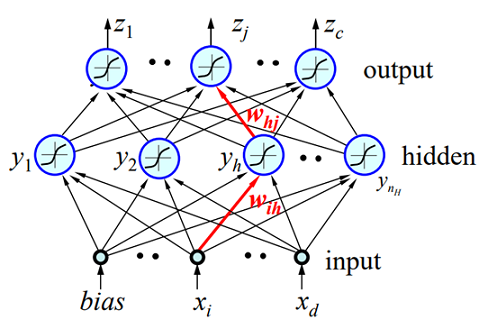
\includegraphics{Images/fig1.jpg}}
\caption{Classical three-layer neural network}
\label{fig}
\end{figure}
对上图所示的一个三层神经网络,当Activation Function选用$Sigmoid$时,其反向传播(BP)过程中,
待更新的权重有两个$w_{hj}$和$w_{ih}$,他们各自的增量$\Delta w_{hj}$和$\Delta w_{ih}$
可以由公式表示:
$$
\delta_{j}^{k}=\frac{-\partial E}{\partial n e t_{j}^{k}}
=f^{\prime}\left(n e t_{j}^{k}\right)\left(t_{j}^{k}-z_{j}^{k}\right)
=z_{j}^{k}\left(1-z_{j}^{k}\right)\left(t_{j}^{k}-z_{j}^{k}\right)
$$
$$
\delta_{h}^{k}=\frac{-\partial E}{\partial n e t_{h}^{k}}
=f^{\prime}\left(n e t_{h}^{k}\right) \sum_{j} w_{h j} \delta_{j}^{k}
=f^{\prime}\left(n e t_{h}^{k}\right) \Delta_{h}^{k}
$$
$$
\Delta w_{ih}=\eta \sum_{k}\left(f^{\prime}\left(n e t_{h}^{k}\right) 
\sum_{j} \delta_{j}^{k} w_{h j}\right) x_{i}^{k}
=\eta \sum_{k} \delta_{h}^{k} x_{i}^{k}
$$
$$ 
\Delta w_{hj}=\eta \sum_{k}\left(t_{j}^{k}-z_{j}^{k}\right)
f^{\prime}\left(n e t_{j}^{k}\right) y_{h}^{k}
=\eta \sum_{k} \delta_{j}^{k} y_{h}^{k}
$$
式子中,$\delta_{h}^{k}$表示第K个样本$w_{ih}$所连接的边的指向结点(隐含结点h)
收集到的误差信号;$\delta_{j}^{k}$表示$w_{hj}$所连接的边的指向结点(输出节点)的误差信号,
而误差大小等于该结点收集到的误差乘以激励函数对“该结点加权和”的导数,即为$\Delta w_{ih}$和
$\Delta w_{hj}$,再由$w = w + \Delta w$对权重进行修正。
\par
$\mathbf{Q2}$:请描述自组织映射网络的构造原理,给出自组织算法的计算步骤(即网络训练)。\par
$\mathbf{A1}$:自组织算法,又称Self-organizing map$(SOM)$算法,是一种无监督的人工神经网络。它给同一层的神经
网络节点引入了竞争机制,通过神经网络相近邻的节点间进行侧向交互作用彼此竞争,自适应地学习成为具有不同功能网络
分区的神经网络结构。它可以实现在不知道类别的情况下,对数据进行聚类;可以识别针对某问题具有内在关联的特征。\par
\begin{figure}[htb]
\centerline{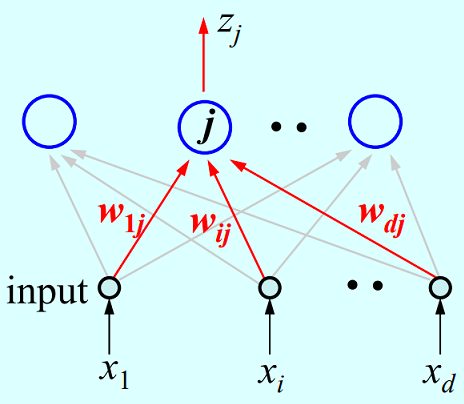
\includegraphics{Images/fig2.png}}
\caption{Typical SOM three layers network}
\label{fig2}
\end{figure}
\begin{enumerate}[$\mathbf{A2}$:SOM网络的训练过程可以列为:]
\item 初始化网络,采用随机初始参数输入。
\item 输入向量值。
\item 计算输入向量至各个映射层的权重向量的距离:
$$
d_j = \sqrt{\sum_{i=1}^{d}(x_i-w_{ij})^{2}}
$$
\item 比较各个神经源的距离值,对比筛选出最小距离的神经源作为胜出神经元将它与附近的神经源做一个递减
的激活,并计算相应的权重改变量:
$$
\Delta w_{ij} = \eta h(j,j^*)(x_i - w_{ij})$$ 
$h(j,j^*)$项为距离权重修正(又称邻域函数),其大小为:
$$
h(j, j *)=\exp \left(-\left\|j-j^{*}\right\|^{2} / \sigma^{2}\right)
$$
它本质上就是以获胜神经元为中心做了一个胜出领域,对胜出领域的神经源进行赋权。
\item 按下式修正权重向量:
$$
w_{ij}^{k+1} = w_{ij}^{k} + \Delta w_{ij}
$$
\item 随着权重值的不断迭代修正,胜出领域的不断缩小,输入向量后仅仅会激活获胜神经源与其附近极个别的
神经源,实现了无监督条件下的聚类操作。因此,学习方法是一种从粗调整向微调整变化,最终达到预定目标的过程。
\end{enumerate}
\end{CJK}

\section{Programming}
\begin{CJK}{UTF8}{gkai}

$\mathbf{Q1}$:请编写两个通用的三层前向神经网络反向传播算法程序,一个采用批量方式更新权
重,另一个采用单样本方式更新权重。其中,隐含层结点的激励函数采用双曲正切
函数,输出层的激励函数采用 sigmoid 函数。目标函数采用平方误差准则函数。 \par
$\mathbf{A}$:我们采用了基于$Tensor Flow$的$keras$模块,代码均由$Python$编译,
我们的网络隐藏节点数为3,学习率$lr=0.1$,迭代次数$epchos=80$,程序运行的结果图如Fig2所示:
\begin{figure}[htb]
\centerline{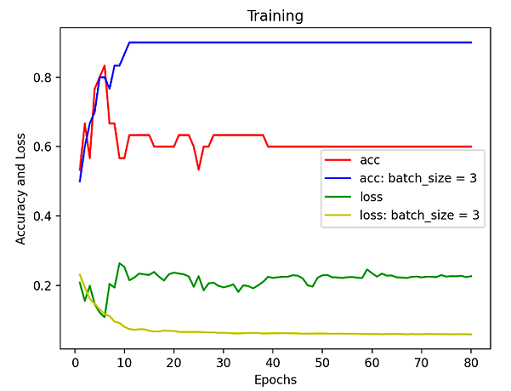
\includegraphics{Images/fig3.png}}
\caption{The training result in Batch=3 or Batch=1}
\label{fig3}
\end{figure}
从结果图中可以明显看出,采用$Batch$的组收敛速度远高于未使用$Batch$的组。此外,不使用$Batch$的组
的训练正确率$acc$和损失$loss$的震荡十分严重,$Batch$的引入明显降低了训练过程中的波动,优化了计算结果。

$\mathbf{Q2}$: (a)隐含层不同结点数目对训练精度的影响;(b)观察不同的梯度更新步长对训练的影响,并给出一些描述或解释;
(c)在网络结构固定的情况下,绘制出目标函数值随着迭代步数增加的变化曲线。 \par
$\mathbf{A1}$:由Q1的讨论,我们选取了更加稳定和易收敛的使用$Batch$的模型作为验证对象。我们选用的学习率$lr=0.1$,
隐藏层节点数$Hidden nodes$分别是3,6,9。循环次数$epochs=100$。程序运行结果如下图所示: \par
\begin{figure}[htb]
\centerline{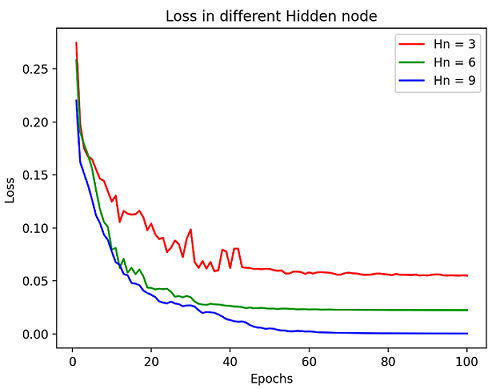
\includegraphics{Images/fig4.png}}
\caption{The training result in different Hidden nodes}
\label{fig4}
\end{figure}
可以看出,采用$Batch=3$的$liner$模型,其精度随着隐藏层节点的上升而提高,且隐藏层节点较少时,
其误差输出出现明显的波动。但另一方面,采用高节点的网络因为其复杂程度的上升,收敛速度往往会
慢于低节点数的网络,这也启示我们在使用神经网络计算时应当挑选合适的节点数目。\par
$\mathbf{A2}$:我们选取了学习率($\eta = 0.1,0.2,0.3$)作为我们的测试对象。$Hidden node=6$,
其余设置与A1的设置类似。程序的输出结果如下: \par
\begin{figure}[htb]
\centerline{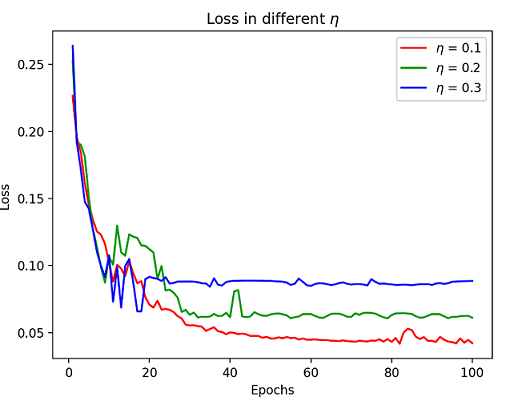
\includegraphics{Images/fig5.png}}
\caption{The training result in different learning rates}
\label{fig5}
\end{figure}
可以看出,不同的学习率对程序的收敛和训练结果存在较大影响。较大的学习率虽然可以使得程序快速
收敛,但也往往容易陷入局部区间,训练损失大,训练效果差;较小的学习率收敛速度较慢的同时,也具有
相对较好的平滑性与训练结果。造成这种差异的原因主要在于学习率$\eta$的大小直接关系到网络中
各个参数的更新步长,对神经网络的更新存在直接关系。在日常的实验中,选取合适的学习率至关重要。 \par
$\mathbf{A3}$:在这一问中,我们选取了表现较好的模型$\eta=0.1,batch=3,Hidden node=6$来训练,
训练的损失随迭代次数$epochs$的变化如下图:   \par
\begin{figure}[htb]
 \centerline{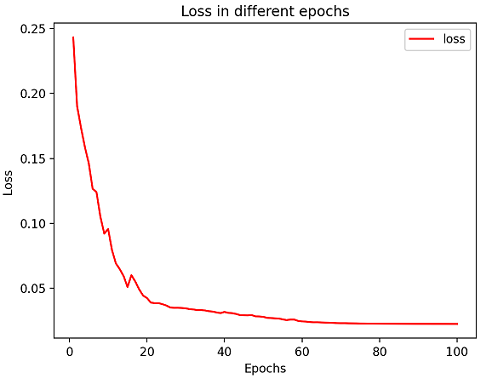
\includegraphics{Images/fig6.png}}
\caption{The training result in different epchos}
\label{fig6}
\end{figure}
可以看出,使用了$Batch$技术的模型收敛效果无论是光滑性还是速度都较好;训练的损失随着$epochs$的增加
稳步下降,偶尔会存在很小的波动;模型整体在$epochs=80$附近收敛,继续训练模型的loss变化较小。

\end{CJK}

\section{Appendix}
\begin{CJK}{UTF8}{gkai}
    本次作业中,所采用的拟合计算代码均是基于Matlab和Python3.9,相关的源码已经被开源于Github上:
    \url{https://github.com/Alexiopro/First-year-of-UCAS/tree/main/UCAS/Source%20Code%20of%20Pattern%20Classification}
    供读者查用。 \par
\end{CJK}
\end{document}
